\chapter{Rate of SLSNe at z$\sim$1}
\label{Chapter4}
\lhead{Chapter 4. \emph{Rate of SLSNe}}

The rate of any transient event is one of its most fundamental properties, providing clues about their origin and evolution throughout the history of the universe. In this chapter I present the measurement of a volumetric rate of SLSNe at z$\sim$1 measured using the archival SNLS data, providing a unique opportunity to test their progenitor models. Since their identification, SLSNe have been known to be an extremely rare class of events. The low rate suggests that the origin of SLSNe must be connected with an equally rare progenitor scenario. The motivation behind our measuring is to study the evolution of the rate by bridging the gap between the local and high redshift measurements of the rate.

Prior to this work, there were three published measurements of the rate of SLSNe. A local rate of was calculated using a single SLSN-I event discovered by the Texas Supernova Search (TSS) \citep{Quimby2014}, giving a value of $\rho_{\mathrm{SLSN}} = 19^{73}_{17}$ SNe Gpc$^{-3}$ Yr$^{-1}$ at the volume weighted redshift of z=0.23. The large measurement uncertainty can be attributed to the Poissonian statistics of their scarce sample as well as the uncertainty in the detection efficiency driven by the diversity of SLSN population. In contrast to the local value, \citet{Cooke2012} presented a rate of SLSNe at a volume-weighted z$\sim$3 using two SLSNe discovered in the deep stacked SNLS data. They estimate $\rho_{\mathrm{SLSN}}$ = 400 SNe Gpc$^{-3}$ Yr$^{-1}$, however, do not provide an uncertainty estimate which we must assume, making a conservative estimate to be 50\%. The final of the three measurements was performed by \citet{McCrum2014} using a sample of spectroscopically confirmed SLSNe in the PanSTARRS. This measurement, however, used a different approach basing the rate of SLSNe on the relative rate and spectroscopic completeness with respect to CCSNe discovered in the same data set. While I include this measurement for comparison purposes, the values cannot be directly related.

None of the above experiments measures the rate in the region of z$\sim$1, leading to a gap near to the peak of the star formation history of the universe. This region is particularly interesting to us, not only as there is a large number of SLSNe detected at that redshift, but also as a test for a number of progenitor theories. The rate measured in that volume is fundamental in order to establish whether the rate of SLSNe follows that of the star formation history of the Universe. Demonstrating this could give further evidence to support the models where the birth of a SLSN is connected to a death of a very massive and therefore young progenitor.

SNLS provides a great dataset for this project. With detecting high redshift SNIa as one of its main goals, the SNLS dataset is full of deep and high-quality light curves. The survey has already serendipitously discovered two, high redshift, SLSN \citep{Howell2013} making it a safe choice while simultaneously having a potential to hide more, not yet identified objects. This work follows a series of similar measurements performed using the same dataset. The rate of SNIa, as well as the point source detection efficiencies, were found by \citet{Perrett2012}. The rate of CCSN was measured by \citet{Bazin2009}, providing a unique opportunity to compare the rate of SLSNe and CCSN using a deep, homogeneous dataset.

The order of this chapter is as follows. First, I propose a photometric definition of SLSNe based on the modelling of their light curves using the spin-down of a magnetar model followed by a search for missed objects within the SNLS dataset. I briefly introduce the photometric sample of SNLS SLSNe before describing the Monte Carlo simulation used in order to measure the rate and its uncertainties. Finally, I compare the value measured to the previously published results and discuss its significance in terms of the physical origin of the objects as well as their detectability by DES and future surveys. The work presented in this chapter has been published in \citet{Prajs2016}.

\section{Defining a SLSN}
\label{sec:SLSNDefinition}
The first task in the process of measuring the rate of SLSNe was to develop a method for the photometric selection of optical transients that were to enter our SLSN sample. The earliest definitions of SLSNe relied on their peak luminosity and often defined them as SN with an absolute $u$-band magnitude of $M_{u}<-21$ \citep{Gal-Yam2012}. This definition is not adequate for our search for two main reasons. Firstly, after that definition was formulated, several examples of events that are spectroscopically similar to SLSNe but that do not pass this arbitrary threshold have been discovered. Some of these events included DES13S2cmm \citep{Papadopoulos2015} and LSQ14mo \citep{Leloudas2015a} which both have M$_u$ > -21 despite being spectroscopically consistent with SLSNe and are associated with a very slow light curve evolution. Secondly, a new class of fast and luminous transients with luminosities similar to SLSNe but with a faster light curve evolution as well as different spectroscopic types has recently been discovered \citep{Arcavi2016}. Instead of an arbitrary luminosity cut, I use a photometric classification approach based on the modelling of SLSNe using the spin-down of a magnetar model as a simple analytical model that provides a good fit to a sample of confirmed SLSNe.

This approach to classifying SLSNe did have several drawbacks. The use of an analytical model implied that the rate was calculated only for objects which are similar to the sample of confirmed SLSNe, as presented in \sref{sec:litSample}. It was clear, at the time this work was undertaken, that this would likely not capture all objects of this class. Without a better definition of a SLSN more significant progress could not be achieved. In \cref{Chapter5} I present a more sophisticated and complex approach to this problem, based on an artificial training sample of SLSNe and Machine Learning classifiers, before applying it to DES. In the meantime, however, this work presents a rate of SLSNe based on the best data available at the time that the work was undertaken and measures the rate of a 'classic' or the original sample of SLSN with M$_u~\ltsim $~-21.

\subsection{Modeling SLSNe}
In order to model SLSN, I required two main ingredients: an underlying model for the time-dependent bolometric luminosity of a SLSN and an SED that can convert this bolometric luminosity into time-evolving spectra. This together forms a spectral series from which we can synthesise the photometry in any desired filter and at any desired redshift. This can then be used for comparison to observed data. For the purpose of this chapter, the exact form or the physical meaning behind the light curve model parameters are irrelevant as, in practice, any model that satisfactorily replicates the observables could be used for this purpose. I, therefore, provide only a brief overview of the model here while the remaining details are described in \sref{sec:SLAP}.

\subsubsection{Magnetar model}
The spin-down of a magnetar model assumes that a collapse of a giant star with an initial mass of M $>$ 40M$_{\odot}$ produces a SNIc like explosion whilst giving birth to a magnetar; a highly magnetized neutron star with a rotation period on the timescale of milliseconds \citep{Kasen2009,Woosley2010,Inserra2013}. The simple toy model assumes a spherically symmetric ejecta and a constant opacity. The free parameters in the model are the time of explosion, $t_{\mathrm{expl}}$, the magnetic field, $B_{14}$, spin period, $P_{\mathrm{ms}}$ and the diffusion timescale $\tau_M$ which is directly proportional to the ejecta mass, M$_{\mathrm{ej}}$.

\subsubsection{Fitting literature light curves}
The magnetar model provides a good fit to all the SLSNe that form part of our training sample. \tref{table:Magnetar} contains the model's best-fit parameters, as well as two additional derived observables which help us to identify the nature of the events without visually inspecting the light curves. These are the peak absolute magnitude in the SDSS $u$-band filter as well as the rise-time, $t_\mathrm{rise}$, of the SN as measured from the explosion to maximum light in the rest-frame $u$-band. It is important to note here that the absolute magnitude, $M_u$, are given in the AB magnitude system. The zero-point correction factor between the AB and Vega magnitude system for the $u$-band filter is: $M_u^{\mathrm{AB}}\simeq M_u^{\mathrm{vega}}+0.9$ \citep{Blanton2007}. Therefore, while some of the training samples have $M_u^{\mathrm{AB}}>-21$, none have $M_u^{\mathrm{vega}}>-21$ which agrees with the previous definition of a SLSN.

\begin{table}
\begin{center}
\caption{Magnetar model parameters for the sample of 15 published SLSNe.}
\label{table:Magnetar}
\begin{tabular}{|l|r|r|r|r|r|r|r|r|r|r|}
\hline
  \multicolumn{1}{|c|}{Name} &
  \multicolumn{1}{c|}{$M_u$} &
  \multicolumn{1}{c|}{$t_\mathrm{rise}$} &
  \multicolumn{1}{c|}{$\tau_\mathrm{m}$} &
  \multicolumn{1}{c|}{$B_{14}$} &
  \multicolumn{1}{c|}{$P_{\mathrm{ms}}$} &
  \multicolumn{1}{c|}{$t_\mathrm{expl}$} &
  \multicolumn{1}{c|}{$E(B-V)$} &
  \multicolumn{1}{c|}{$\chi^2_{\nu}$} &
  \multicolumn{1}{c|}{Template} \\ & &
  \multicolumn{1}{c|}{(days)} &
  \multicolumn{1}{c|}{(days)} &
  \multicolumn{1}{c|}{($\times10^{14}$ G)} &
  \multicolumn{1}{c|}{(ms)} &
  \multicolumn{1}{c|}{(MJD)} & \\
\hline
  PTF12dam & -21.4 & 34.72 & 22.15 & 0.78 & 2.85 & 56044.5 & 0.18 & 2.49 & 06D4eu\\
  SN2011ke & -21.2 & 24.84 & 30.61 & 3.67 & 2.13 & 55647.5 & 0.01 & 1.31 & iPTF13ajg\\
  SN2010gx & -21.7 & 24.56 & 30.36 & 3.20 & 1.54 & 55247.1 & 0.19 & 0.86 & 06D4eu\\
  SN2013dg & -21.2 & 25.37 & 28.05 & 3.30 & 2.75 & 56412.3 & 0.07 & 0.23 & SCP06F6\\
  PS1-11ap & -21.8 & 32.1 & 20.08 & 0.79 & 2.51 & 55559.0 & 0.02 & 1.62 & 06D4eu\\
  DES14X3taz & -21.7 & 47.21 & 26.16 & 0.23 & 1.67 & 57019.2 & 0.09 & 5.18 & 06D4eu\\
  PS1-10bzj & -21.2 & 22.17 & 18.44 & 2.65 & 3.84 & 55524.0 & 0.07 & 0.37 & 06D4eu\\
  DES13S2cmm & -20.0 & 30.7 & 21.19 & 1.28 & 5.29 & 56509.0 & 0.01 & 0.51 & 06D4eu\\
  iPTF13ajg & -22.4 & 31.45 & 33.41 & 1.57 & 1.32 & 56346.9 & 0.19 & 0.30 & iPTF13ajg\\
  07D2bv & -21.1 & 28.41 & 36.88 & 3.40 & 2.18 & 54132.4 & 0.05 & 0.41 & SCP06F6\\
  06D4eu & -21.9 & 21.48 & 29.94 & 3.82 & 1.00 & 53956.3 & 0.11 & 1.26 & 06D4eu\\
\hline\end{tabular}
\end{center}
\end{table}

\subsubsection{Defing a SLSN parameter space}
\fref{fig:SLAPparam} shows the best-fit magnetar model parameter space. In order to define a region of the parameter space that defines a SLSN, I enclosed the cluster of our literature points with an ellipsoid. I chose it as the lowest volume, simple geometric body that was consistent with all the SLSN in our training sample. The ellipsoid is defined in terms of the three main fit parameters of the magnetar model, $\tau_\mathrm{m}$, $B_{14}$ and $P_{\mathrm{ms}}$. In the Cartesian coordinate system, a position on any generic ellipsoid can be defined using \eref{eq:Ellipsoid}.

\begin{equation}
\label{eq:Ellipsoid}
\left( \begin{matrix}
x \\
y \\
z
\end{matrix} \right)
=
\mathbf{A}
\left( \begin{matrix}
R_x\cos(u)\cos(v) \\
R_y\cos(u)\sin(v) \\
R_z\cos(v)
\end{matrix} \right)
+ \mathbf{C}
\end{equation}

\noindent where \textbf{A} is a rotation matrix, \textbf{R} is the radius of the ellipsoid and \textbf{C} is the position of its center. The following conditions must be satisfied: $-\pi /2 \leq u \leq \pi /2$ and $-\pi \leq v \leq \pi$. I have set up our parameter space such that $\tau_\mathrm{m}$ lays along the $x$-axis, $B_{14}$ is along the $y$-axis and $P_{\mathrm{ms}}$ corresponding to the $z$-axis. Using the Khachiyan Algorithm \citep{Aspvall1980,Khachiyan1980}, I performed an analytical fit to determine the ellipsoid that best describes the known population of SLSNe, founding the best-fit ellipsoid to have the following properties:

\begin{equation}
\label{eq:A}
\mathbf{A} =
\left( \begin{matrix}
-0.184 & 0.575 & -0.797\\
 0.008 & 0.812 & 0.586\\
0.983 & 0.102 & -0.154
\end{matrix} \right)
\end{equation}

\begin{equation}
\label{eq:R}
\mathbf{R} =
\left( \begin{matrix}
R_x \\
R_y \\
R_z
\end{matrix} \right)
=
\left( \begin{matrix}
1.89\\
2.17\\
11.32
\end{matrix} \right)
\end{equation}

\begin{equation}
\label{eq:C}
\mathbf{C} =
\left( \begin{matrix}
26.76 \\
2.14\\
2.77
\end{matrix} \right)
\end{equation}

\noindent \fref{fig:SLAPparam} shows the three, two-dimensional projections of this parameter space, populated with our training sample of literature SLSNe.

\begin{figure}
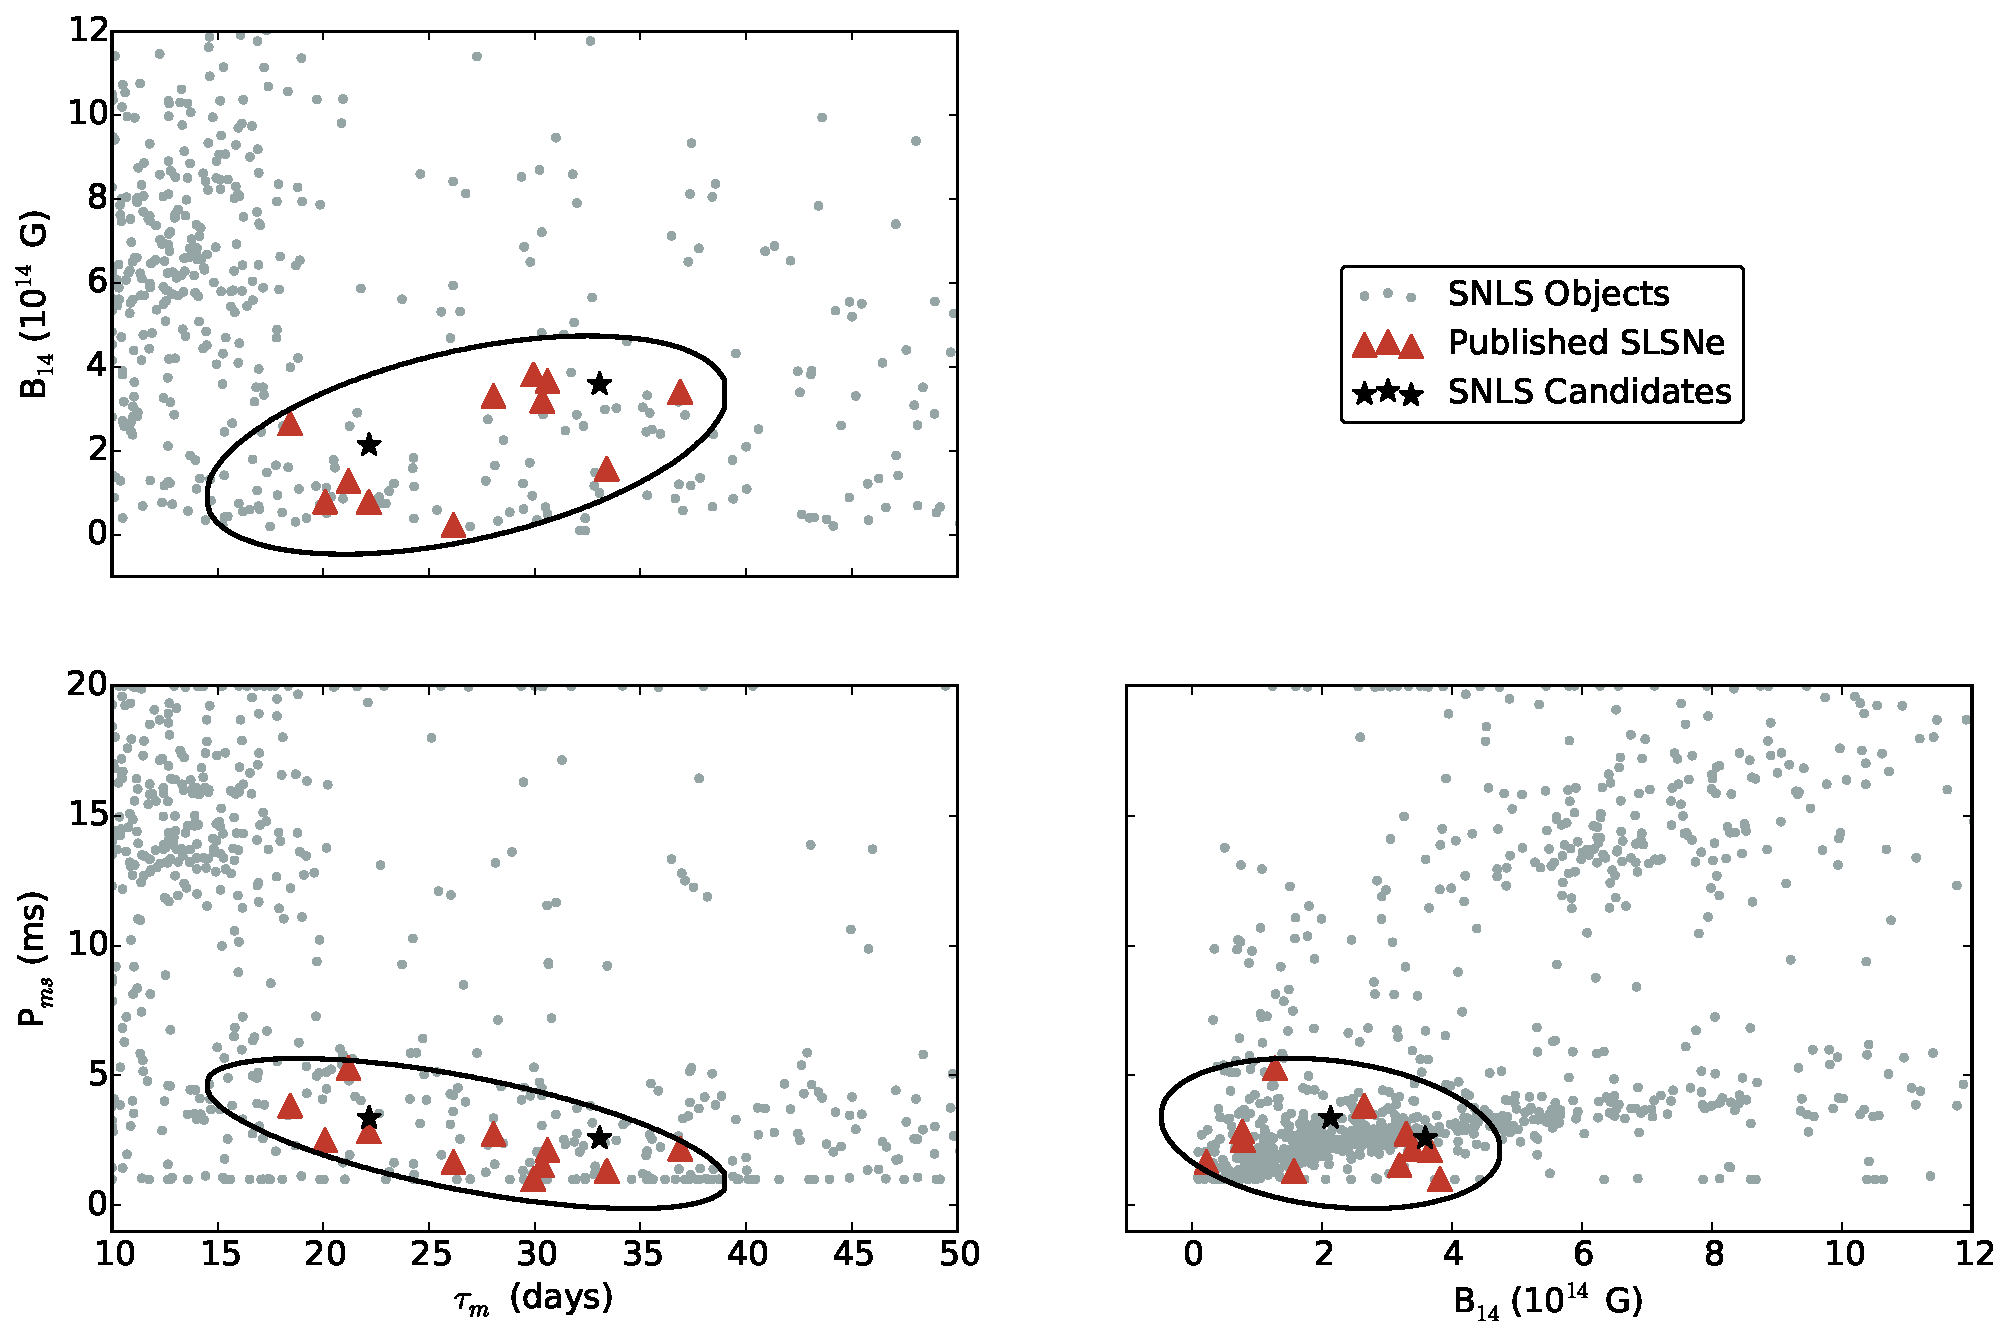
\includegraphics[width=\textwidth]{Figures/Chapter4/SLAPparam}
\caption{The $\tau_\mathrm{m}$--$B_{14}$--$P_{\mathrm{ms}}$ parameter space constructed from the magnetar model fits. The SNLS objects are denoted by grey circles. The ellipses correspond to the two-dimensional projections of the three-dimensional ellipsoid, fitted around the parameter space of the known SLSNe (shown as triangles) to form a region defining them in terms of the model. The SNLS candidates that fall within this parameter space are shown as stars.}
\label{fig:SLAPparam}
\end{figure}

\section{Searching for SLSN in SNLS}
Having formed a photometric definition of SLSNe in \sref{sec:SLSNDefinition}, I now proceed to describe the steps undertaken in order to identify any potential missed SLSNe in SNLS. My approach was based on fitting the magnetar model to SNLS light curves and comparing their best-fits to the parameter space defined by the training sample. In the ideal case we would first like to test the definition against an independent test sample of objects that were not used in forming the definition. Unfortunately, the number of known SLSN events at that time was too low to allow us to afford to split it into a training and test samples. I therefore make the assumption that the parameter space in \fref{fig:SLAPparam} is defined by a representative sample of events. This provides a further motivation to seek a more elegant and robust solution for any future search of SLSN such as the one performed on the DES dataset in \cref{Chapter5}. I would also like to note that both the fitting method and the definition of a SLSN-like event presented in this chapter do not makes any assumption about the luminosity of the event. This makes it entirely possible for fitted events to have $M_u>-21$ and still be classified as SLSNe, broadening the current definition of SLSN into potentially previously unexplored parts of the parameter space. Furthermore, the inverse is also true where some events with $M_u<-21$, including those with a relatively short diffusion timescale, $\tau_\mathrm{m}$, giving rise to a faster evolution, are shown to be inconsistent with SLSNe. This natural consequence of the technique used here is should therefore lead to a purer sample of SLSNe than a arbitrary magnitude cut.

\subsection{Magnetar model fitting}
With the model and definition of SLSNe in place, my next task was to apply the same technique to the sample of SNLS transients. The SNLS detected 4949 transient objects in total \citep{Perrett2010}. This included many objects that were visually designated as active galactic nuclei (AGN) and variable stars, as well as supernovae. In order to perform the fitting on the sample, I first matched each object with a redshift where known. 1694 objects in the transient catalogue have spectroscopic redshifts, either from spectra of the transients or of the host galaxy. The redshift association here is trivial as the spectroscopic measurements directly target either the SN or its host galaxy.

As previously described in \sref{sec:SNLSRedshift}, where a spectroscopic redshift is not available, I use photometric redshift estimates. SNLS transients were associated with potential host galaxies by selecting the nearest galaxy within a radius of 1.5''. [MARK: DO I NEED TO EXPAND ON WHY WE MADE THIS CUT?] This provided photometric redshift information for a further 1527 events. As the photometric redshift estimates are less precise than their spectroscopic counterparts I do not use them directly. Instead, I iterate over a range of redshift values spanning the photometric redshift uncertainties between the lower to upped uncertainty band in steps of $\Delta$z = 0.04.

At this stage of the analysis, 1728 candidates remain with no redshift information. Due to the difference in depth of the SNLS deep stack compare to that of the science images we expected fewer objects to be considered as 'hostless' in the sample since SNLS should be able to measure photometric redshifts for all but the very faintest host galaxies. I carried out an inspected these objects both visually and using simple statistics (including the number of detected bands, number of detections per band and the time elapsed between detections) and found that a large number of these objects were, in fact, likely to be false detections that incidentally matched the SNLS real-time detection criteria \citep{Perrett2010}. This inspection showed that only 292 of these objects have multiple detections in multiple bands and are therefore likely to be real. For this remaining sample, I iterate over a broad range of redshifts (0.2 $\leq$ z $\leq$ 1.6 in steps of $\Delta$z = 0.1) but otherwise treat them identically to objects with a known redshift.

Once the events were associated with their respective redshifts, I then proceed to fit the SNLS sample to the magnetar model. During the fitting process, I apply the same quality cuts as for the SLSN training sample. I have excluded objects with less than two detections in at least three bands between the best-fit explosion date and maximum light, and a further two detections in at least three filters between maximum light and $+30$ days. For the purpose of this work, I consider a detection to be $\geq5$\,$\sigma$ in the real-time photometry. Amongst the 4949 SNLS transients only 2097 pass the final data quality cuts. Their best-fits to the magnetar model are shown in \fref{fig:SLAPparam}.

\subsection{Candidates}
\label{sec:SLSNCands}
While the magnetar model is known to be very flexible, allowing for a variety of light curve morphologies, it has proven not be a good fit for the majority of the SNLS objects. A simple $\chi^2$ test is sufficient to remove a large number of these poor fits quality objects. I apply a conservative cut at a $\chi^2$ per degree of freedom ($\chi^2_{\nu}$) of 20. I chose such a large value of $\chi^2_{\nu}$ in order to retain all SLSNe, including these that might be associated with pre-peak 'bumps' \citep{Nicoll2016,Nicoll2015a,Smith2016}. Such objects are well represented by the magnetar model in the 'main' part of the event, however, due to the extra undulations, their goodness-of-fit is not ideal when taking into account a full season light curve.

Of the SNLS objects that pass our data quality and $\chi^2_{\nu}$ cuts, four lied within the parameter space of SLSNe as defined in \ref{sec:SLSNDefinition}. This includes the two spectroscopically confirmed events from \citet{Howell2013} that were part of our training sample. For the other two candidates, SNLS-05D3ks and SNLS-07D3bs, I  measured the multi-season light curves using the custom \textsc{PTFPHOT} pipeline (described in \cref{Chapter2}) to allow us to visually inspect the objects and search for signatures of any long-term variability or detections prior to, or sufficiently after, the putative supernova event. This process of visual inspection eliminates SNLS-05D3ks which shows clear multiple maxima spanning three years as seen in \fref{fig:05D3ks}, leaving us with just a single, new SLSN-like candidate: SNLS-07D3bs.

\begin{figure}
\centering
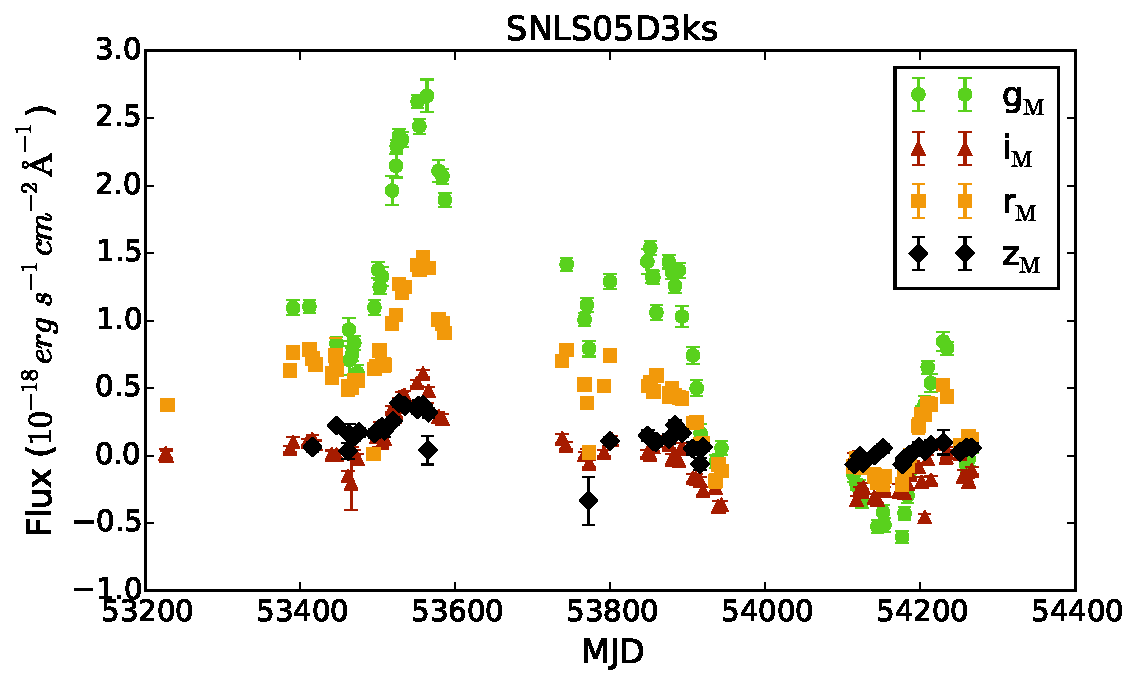
\includegraphics[width=\textwidth]{Figures/Chapter4/SNLS05D3ks}
\caption{The $g_M$, $r_M$, $i_M$, $z_M$ multi-season light curve of SNLS-05D3ks. This transient is found within the SLSN parameter space (\fref{fig:SLAPparam}), but does not pass visual inspection as it shows clear signs of multiple maxima.}
\label{fig:05D3ks}
\end{figure}

\subsection{SNLS-07D3bs}
\label{sec:07D3bs}
SNLS-07D3bs is identified as a SLSN candidate between $0.6<z<1.2$ based on its host galaxy photometric redshift estimate. The best-fit magnetar model for the object is obtained at z = 1.0. While SNLS-07D3bs was never classified or recognised as an object of interest during the life of SNLS, it has been spectroscopically observed on the 17$^{\mathrm{th}}$ April 2007 using the Keck/LRIS instrument. This data was never published officially as no spectral classification was obtained at that time. The data was however presented in a PhD thesis by \citet{Fakhouri2013}.

At the time the observations of SNLS-07D3bs were made, the SLSN class was not yet known and no SLSN spectral templates were available for comparison with the data. It is also because of this that the SLSN that have been previously identified in SLSN by \citet{Howell2013} have not been originally identified as objects of interest until several years after their initial detection. Using the \textsc{superfit} spectrum identification tool \citep{Howell2005}, the spectrum of SNLS-07D3bs was re-analysed by fitting all available SN templates at a broad range of redshifts exceeding our photometric estimate. The data are noisy with a signal-to-noise $\sim$ 7 as observing conditions were quite poor. Despite this, I find the best spectral match to be to the SLSN iPTF13ajg at $z=0.757$ as can be seen in \fref{fig:07D3bsSpec}. While this is clearly an uncertain spectral classification, there is no evidence from the spectrum that the object is not a SLSN, particularly as the best match is an event of that type. The magnetar model also provides a good fit at that redshift as seen in  \tref{tab:07d3bsParams}. The host galaxy, located at RA=14h~21m~50.466s, Dec=+53$^{\circ}$~10'~28.58'', is detected in the SNLS deep stack images \citep{Ilbert2006}, but is very faint, with AB magnitudes of ($u_M$, $g_M$, $r_M$, $i_M$, $z_M$) = ($26.61\pm0.49$, $26.13\pm0.16$, $25.67\pm0.13$, $25.18\pm0.11$, $25.19\pm0.37$). Combining the spectral and magnetar model fitting, as well as a faint host galaxy, matching the properties expected of most SLSNe, provided us with sufficient evidence to consider SNLS-07D3bs to be the third SLSN detected by the real-time pipeline of SNLS.

\begin{figure}
\centering
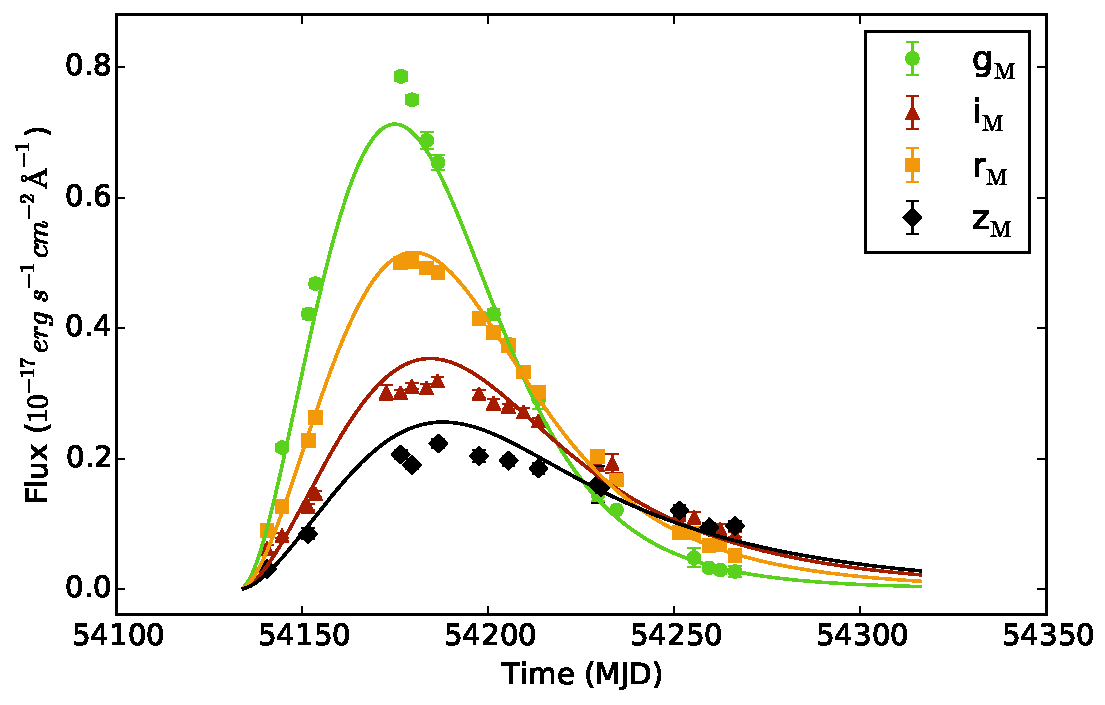
\includegraphics[width=\textwidth]{Figures/Chapter4/07D3bs}
\caption{The $g_M$, $r_M$, $i_M$, $z_M$ light curve of SNLS-07D3bs overplotted with the best-fit magnetar model at $z=0.757$. The candidate shows a good agreement with the model.}
\label{fig:07D3bsLC}
\end{figure}

\begin{figure}
\centering
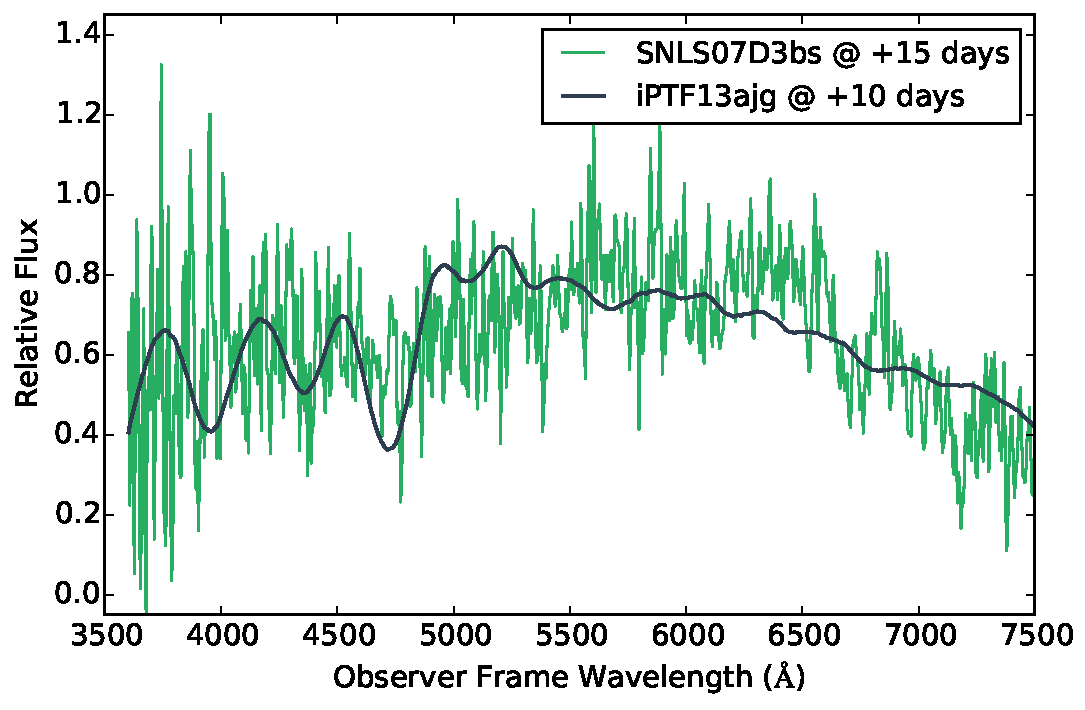
\includegraphics[width=\textwidth]{Figures/Chapter4/07D3bsSpec}
\caption{The spectrum of SNLS-07D3bs from Keck/LRIS, taken 15 rest-frame days after maximum light. The signal-to-noise of the spectrum is low preventing a definitive classification; however, the spectrum is consistent with a SLSN at around $z=0.76$. Weak galaxy emission lines are consistent with $z=0.757$.}
\label{fig:07D3bsSpec}
\end{figure}

\begin{table}
\begin{center}
\caption{Magnetar model parameters for the new SNLS SLSN candidate: SNLS-07D3bs.}
\label{tab:07d3bsParams}
\begin{tabular}{|l|r|r|r|r|r|r|r|r|r|r|}
\hline
  \multicolumn{1}{|c|}{Name} &
  \multicolumn{1}{c|}{$M_u$} &
  \multicolumn{1}{c|}{$t_\mathrm{rise}$} &
  \multicolumn{1}{c|}{$\tau_\mathrm{m}$} &
  \multicolumn{1}{c|}{$B_{14}$} &
  \multicolumn{1}{c|}{$P_{\mathrm{ms}}$} &
  \multicolumn{1}{c|}{$t_\mathrm{expl}$} &
  \multicolumn{1}{c|}{$E(B-V)$} &
  \multicolumn{1}{c|}{$\chi^2_{\nu}$} &
  \multicolumn{1}{c|}{Template} \\ & &
  \multicolumn{1}{c|}{(days)} &
  \multicolumn{1}{c|}{(days)} &
  \multicolumn{1}{c|}{($\times10^{14}$ G)} &
  \multicolumn{1}{c|}{(ms)} &
  \multicolumn{1}{c|}{(MJD)} & \\
\hline
SNLS-07D3bs & -20.9 &  27.2 & 23.7 & 2.28 & 3.81 & 54132.5 & 0.05 & 1.96 & iPTF13ajg\\
\hline
\end{tabular}
\end{center}
\end{table}

\section{The rate of superluminous supernovae}
\label{sec:MC}
In the previous sections, I have outlined our approach to selecting a suitable definition of SLSNe before applying it to a sample of transient detected by the SNLS. This resulted in identifying a sample of three SLSNe including two previously known objects and a new, previously unclassified example; SNLS-07D3bs. In this section, I describe the method used to calculate the volumetric rate of SLSNe, $\rho_{\mathrm{slsn}}$, implied by these detections. First, I describe the method used for this calculation and the reasoning behind our use of a Monte-Carlo simulation over a purely statistical approach. I then discuss the reasoning behind our choice of the search volume before presenting the rate calculation and the result.

\subsection{Defining a rate}
\label{sec:method}
$\rho_{\mathrm{slsn}}$ can be defined as a sum over the number of SLSNe, $N$, found in a given comoving search volume, $V$, over a search duration, $t$, weighted by the inverse of the detection efficiency, $\epsilon_{i}$, of detecting each event. This can be summerised using \eref{eq:rate}:

\begin{equation}
\label{eq:rate}
\rho_{\mathrm{slsn}} = \frac{1}{V}\sum^{N}_{i}\frac{(1+z_i)}{\epsilon_{i}t_{i}}.
\end{equation}

The factor $(1+z_i)$ corrects for time dilation. The detection efficiency $\epsilon_i$ is a statistic describing how each SLSN should be weighted relative to the whole population. In other words, $1-\epsilon_i$ gives the fraction of similar SLSNe that exploded during the search period but were missed by the survey due to, for example, search inefficiencies. The detection efficiency is a vital and simultaneously the most difficult part of the computation.

\subsection{Detection efficiency}
The full treatment of a detection efficiency for any survey is a very complex problem with many aspects of the survey to be considered including the cadence, image quality, limiting magnitude amongst other. \citet{Frohmaier2017} shows a recent example of such comprehensive study performed with the aim of calculating the local volumetric rate of SNIa in PTF. Our SLSN detection efficiencies are based on a similar analysis by \citet{Perrett2010}, who carried out a study of the detection efficiencies and selection biases of SNIa in SNLS and subsequently calculated a rate of those events in \cite{Perrett2012}. In this study, several million fake SNIa were placed in the SNLS science images, with the correct temporal evolution, and passed through the SNLS real-time detection pipeline. The recovery efficiencies of these SNe Ia could then be estimated. Although these results were produced using a particular model of a particular supernova type, at a more basic level they also provide the recovery efficiencies of point sources in the SNLS data as a function of magnitude in every $i_M$-band image that SNLS took, and it is these more basic data that we use in this study. [MAKE A PLOT SHOWING WHAT THAT LOOKS LIKE FOR A RANDOM OBSERVING EPOCH]

\subsection{Method}
In this work, I reverse the common approach to supernova rate calculations, such as the ones used by \citet{Perrett2012} and \citep{Frohmaier2017}. Instead of calculating the rate of SLSNe starting with the number of detected objects, I calculate the probability that a given initial value of $\rho_{\mathrm{slsn}}$ leads to an eventual detection of three SLSNe in the survey. This method is capable of producing a non-Gaussian uncertainty estimate as a by-product of the calculation as the result is presented in form of a probability distribution (\fref{fig:rateFlat3}). The uncertainties can be simply quoted as the 1$\sigma$ confidence region of this distribution.

To simulate the SLSN population in SNLS, I use a Monte Carlo approach. I 'explode' fake SLSNe randomly within the SNLS search period and search volume, and create artificial SLSN light curves on each epoch corresponding to the SNLS observations, including the effect of $1+z$ time dilation. As a result, it is possible to measure the $i_M$ apparent magnitude on each epoch, which is then compared to the point-source recovery statistics on that epoch to give the probability of detection. I combine all of these individual probabilities to give us an overall detection probability per object.

\subsection{Search volumes}
\label{sec:search-volumes}
The effective SNLS search areas for each field, from which the search volumes can be calculated, was found accurately in \citet{Perrett2012} giving an effective total search area of 3.56\,deg$^2$. The volume is calculated by considering the redshift range to which our search was sensitive. The four observing fields cannot be considered as identical as there are small variation in the detection efficiency amongst the fields. The observing season in the D3 field was longer in comparison to the other fields while D1 and D2 had on average, marginally deeper exposures.

At the low-redshift end, the search volume is set by the redshift at which a SLSN would become saturated in the SNLS data. At the high-redshift end, the volume is set by the redshift at which we are no longer able to recover a SLSN event, i.e. a SLSN would fall below the detection limit of the survey. \fref{fig:zrange} illustrates the redshift range to which the search for SLSNe is sensitive to in SNLS, showing the recovery efficiency as a function of redshift for the three events identified in \sref{sec:SLSNCands}. For events at z $<$ 0.2, the efficiency drops rapidly due to saturation effects setting z = 0.2 as the lower redshift limit. At the upper redshift limit, I choose z = 1.6. Although some events similar to SNLS-06D4eu are detectable at z > 2, the fainter events like SNLS-07D3ds would become undetectable in some of the SNLS search fields at z $<$ 1.6.

\begin{figure}
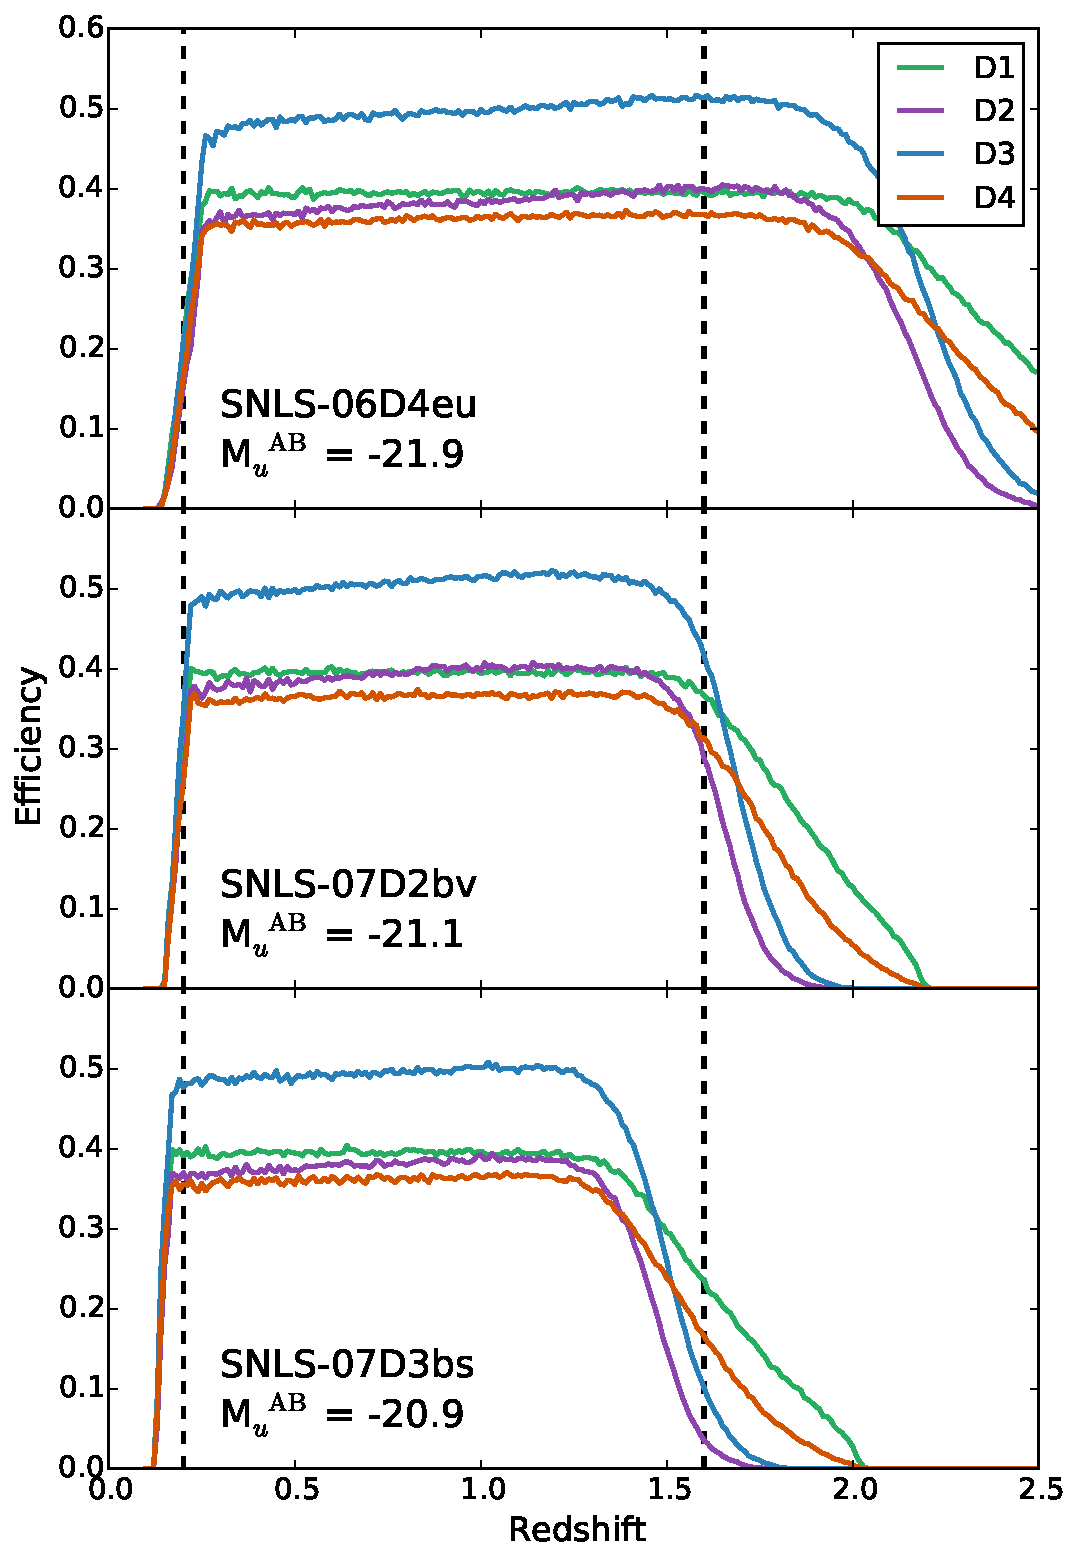
\includegraphics[width=\textwidth]{Figures/Chapter4/Efficiency}
\caption{The redshift range to which our SLSN search is sensitive to, as a function of the four SNLS search fields. The figure shows the recovery efficiency of three different SLSNe as a function of redshift, with each line corresponding to a different search field. The efficiency includes the same data quality cuts as used in the training sample in \sref{sec:Definition} and the SNLS candidate selection in \sref{sec:SLSNCands}. The vertical dashed lines at z = 0.2 and z = 1.6 illustrate the final redshift range used in our Monte Carlo rate calculations.}
\label{fig:zrange}
\end{figure}

\subsection{Monte Carlo simulation}
\label{sec:rate-calculation}
I begin each Monte Carlo simulation with an input $\rho_{\mathrm{slsn}}$ value. From this, I calculate the number of SLSNe that would have occurred within the SNLS search area over the redshift range to which we are sensitive ($0.2<\mathrm{z}<1.6$) in bins of $\Delta$z = 0.01. I assume that this rate does not evolve within the redshift range considered in our simulation. However, this assertion is later tested \sref{sec:SFRRate}. The artificial SLSNe are then assigned a random spatial position (and consequent Milky Way extinction), redshift, host galaxy extinction and physical parameters drawn from the magnetar model parameter space derived from our training sample (\fref{fig:SLAPparam}). A random explosion epoch during the SNLS search period is assigned to each event. From this, the synthetic photometry was calculated on every epoch corresponding to a SNLS observation.

Using the point-source detection efficiencies of \cite{Perrett2010}, I calculate the probability of detecting each SLSN on every epoch of $i_M$ data and combine the probabilities to give the total probability of discovering each object. In order to be considered detected, I enforce that each artificial SLSN must pass the same data quality cuts as both our training sample in \sref{sec:Definition} and our real sample of SNLS candidates in \sref{sec:SLSNCands}. I repeat the entire simulation 100,000 times over an input $\rho_{\mathrm{slsn}}$ range of $5 \leq \rho_{\mathrm{slsn}} \leq 500$\,SNe\,Yr$^{-1}$\,Gpc$^{-3}$.

\fref{fig:rateFlat3} shows the probability of three SLSN events being detected in our simulations as a function of the input rate. A log-normal distribution is fitted to the simulation results and used to smoothly determine the peak of the distribution as well as the 1$\sigma$ confidence regions. From this, we find the rate of SLSNe at z = 1.13, which is the volume-weighted centre of the 0.2 $<$ z $<$ 1.6 range, to be $\rho_{\mathrm{slsn}} = 91^{+76}_{-36}$\,SNe\,Yr$^{-1}$\,Gpc$^{-3}$.

\begin{figure}
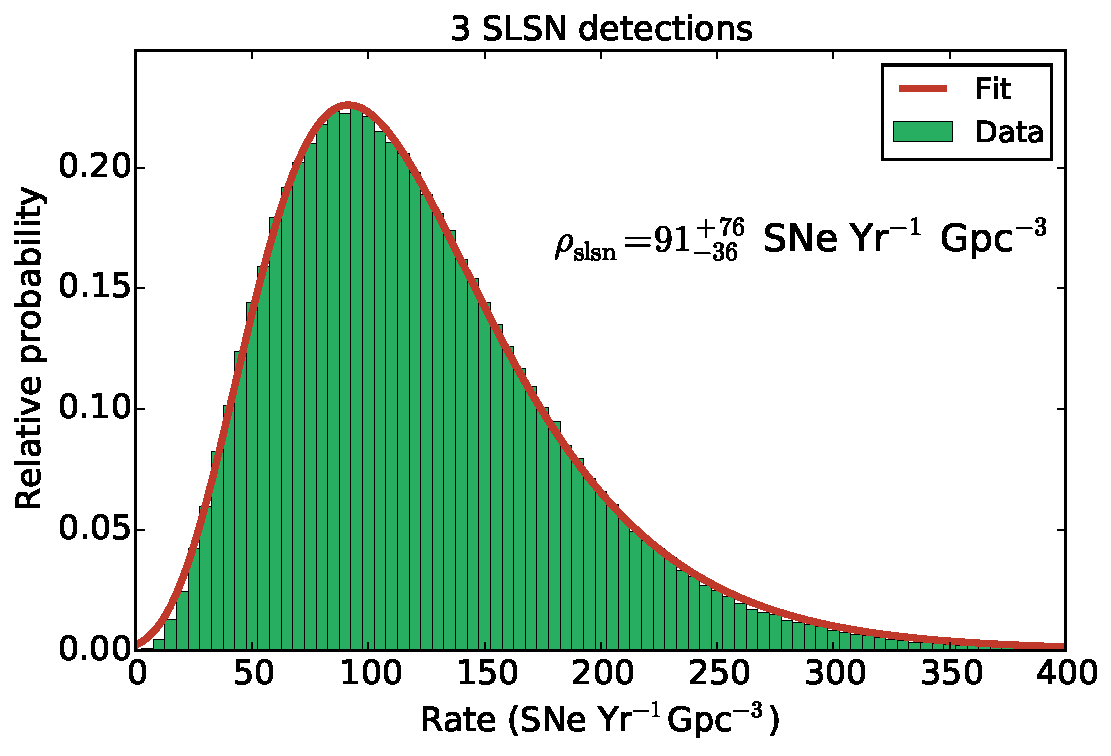
\includegraphics[width=\textwidth]{Figures/Chapter4/rateFlat3}
\caption{The probability distribution of the volumetric rate of SLSNe for the three SLSN candidates over the duration of SNLS at 0.2 $<$ z $<$ 1.6, as determined by our 100,000 Monte Carlo simulations. A log-normal distribution is fit to the data (red line) to estimate the peak of the probability distribution and the uncertainties, quoted as the 68\% confidence region.}
\label{fig:rateFlat3}
\end{figure}

\subsection{Rate assuming a SFR distribution of SLSN}
\label{sec:SFRRate}
As SLSNe are a likely consequence of a collapse of a giant star with an intrinsically fast stellar evolution, it is expected that the rate of SLSNe should follow closely to that of their birth, i.e the cosmic star formation rate. An expected consequence of this would be that a larger proportion of SLSNe are found at high redshift compared with a non-evolving population. I investigate the consequence of this effect on our final rate by repeating the Monte Carlo simulation, instead of drawing the SLSNe from a redshift distribution that follows the cosmic star-formation history as taken from \citet{Hopkins2006} and described in more details in \sref{sec:ConclusionsSFR}. For the value pivoted at z=1.13, as in the case of the flat distribution, I find $\rho_{\mathrm{slsn}} = 98^{+82}_{-39}$\,SNe\,Yr$^{-1}$\,Gpc$^{-3}$. This is very close to the original result and, considering the uncertainties, a negligible difference. Thus our final rate averaged over the redshift range we have considered, is not sensitive to the assumed rate evolution in our simulation. One possible explanation of this is that the relative uniformity of our detection efficiency as a function of redshift within our search volume has negated the effects of the redshift evolution (\fref{fig:zrange}).

\section{Discussion}
Having calculated the rate of SLSNe at an intermediate redshift, it is now interesting to compare the value to other measurements and study its evolution as a function of redshift.

\subsection{Rate Evolution with Redshift}
\label{sec:Discussion}
\begin{figure}
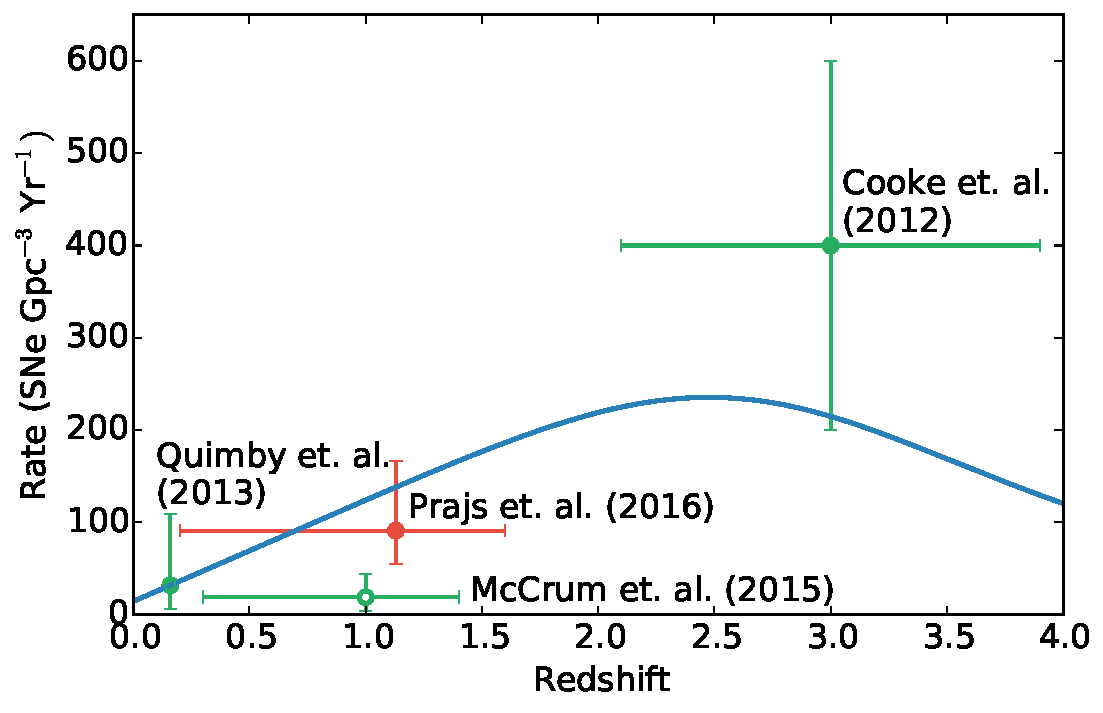
\includegraphics[width=\textwidth]{Figures/Chapter4/rate}
\caption{The evolution of the volumetric SLSN rate as a function of redshift. I compare my measurement to those by \citet{Cooke2012}, \citet{Quimby2014} and \citet{McCrum2014} for comparison. The \citet{McCrum2014} result is marked by an open circle to highlight that it may not be directly comparable with the other measurements as it is derived by a comparison to the rate of core collapse supernovae and is not a direct measurement. The observed evolution is consistent with that of the SFH over the same redshift range; I over-plot in blue the parametrisation of the cosmic SFH of \citet{Hopkins2006}, normalised to the low-redshift SLSN-I rate obtained by \citet{Quimby2014}.}
\label{fig:rate}
\end{figure}

\fref{fig:rate} shows the SLSN rate calculated in this chapter compared with the values published by \citet{Cooke2012}, \citet{Quimby2014} and \citet{McCrum2014}. The volumetric rate increases as a function of redshift with the extent of this observed evolution is consistent with the evolution in the cosmic star-formation history observed over the same redshift range \citep{Hopkins2006}. This is, perhaps, an unsurprising result, as SLSNe are thought to originate from the death of very massive and hence short-lived stars. However, it is important to note here, that we are not able to discriminate between the evolution that follows the star formation history, and one with the same evolution up to $z=1.5$ but followed by a peak at a much higher redshift, as the $z>1.5$ measurement is quite uncertain.

In fact, a higher-redshift peak of the rate may be expected as SLSNe are almost exclusively explode in galaxies that are low-mass, compact dwarfs \citep{Neill2011,Lunnan2015}, and that are metal-poor and strongly star-forming \citep{Chen2013,Lunnan2013,Leloudas2015}. One popular interpretation of this is that the low metallicity must play a role in the formation of SLSNe, which is consistent with the low metal content inferred from their UV spectra \citep{Mazzalli2016}. This scenario would also predict a volumetric rate evolution that follows both the cosmic SFH and cosmic chemical enrichment. The possibility of testing the origins of SLSNe and the role of metal enrichment to their formation gives one of the strongest motivations behind the future studies of their rates at $z>2$.

\subsubsection{Comparison to the rate of CCSN}
Comparing the rate of SLSNe to that of CCSN is yet another particularly interesting test which can inform us about their origin. Using SLSNe discovered by the Pan-STARRS medium-deep survey over $0.3 \leq z \leq 1.4$, \citet{McCrum2014} measure the relative rate of SLSNe to be between $3^{+3}_{-2}\times10^{-5}$ and $8^{+2}_{-1}\times10^{-5}$ that of the core-collapse supernova rate, $\rho_{\mathrm{cc}}$. We use the SNLS $\rho_{\mathrm{cc}}$ measurement at $z\sim0.3$ of $1.42\pm0.6\times10^{-4}$ \,SNe\,Gpc $^{-3}$ \,yr $^{-1}$ \citep{Bazin2009}, and extrapolate it to $z=1.13$, assuming it tracks the cosmic SFH, increasing the rate by a factor of 2.62. Our own absolute SLSN rate can then be expressed as rate relative to that of core-collapse SNe, which we find to be 2.2$^{+1.8}_{-0.9}\times10^{-4}$ of the $\rho_{\mathrm{cc}}$. This is higher than, but still consistent with, the relative rate of \citet{McCrum2014}.

\subsection{Host Galaxies of SNLS SLSNe}
The host galaxies of SLSNe play a key factor in their study. Besides playing a factor in determining their origins they also provide an observable that could act as a further confirmation for a photometrically selected object. \fref{fig:hosts} shows the distribution of SLSN host-galaxy stellar masses as measured by \cite{Lunnan2014}. We use the \textsc{zpeg} photometric redshift package \citep{LeBorgne2002} with the SNLS multi-waveband $g_M$,$r_M$,$i_M$,$z_M$ host galaxy photometry to estimate the stellar mass for SNLS-07D3bs. We are not able to derive host galaxy stellar masses for SNLS-06D4eu and SNLS-07D2bv using the SNLS deep stacks due to the galaxies faintness and the lack of infrared (which correspond to the rest-frame optical) data. We instead use values obtained by \citet{Leloudas2015a} and \citet{Schulze2017}. The host stellar masses for all three of our candidates agree with the published SLSN-I host stellar mass distribution as shown in \fref{fig:hosts}.

\begin{figure}
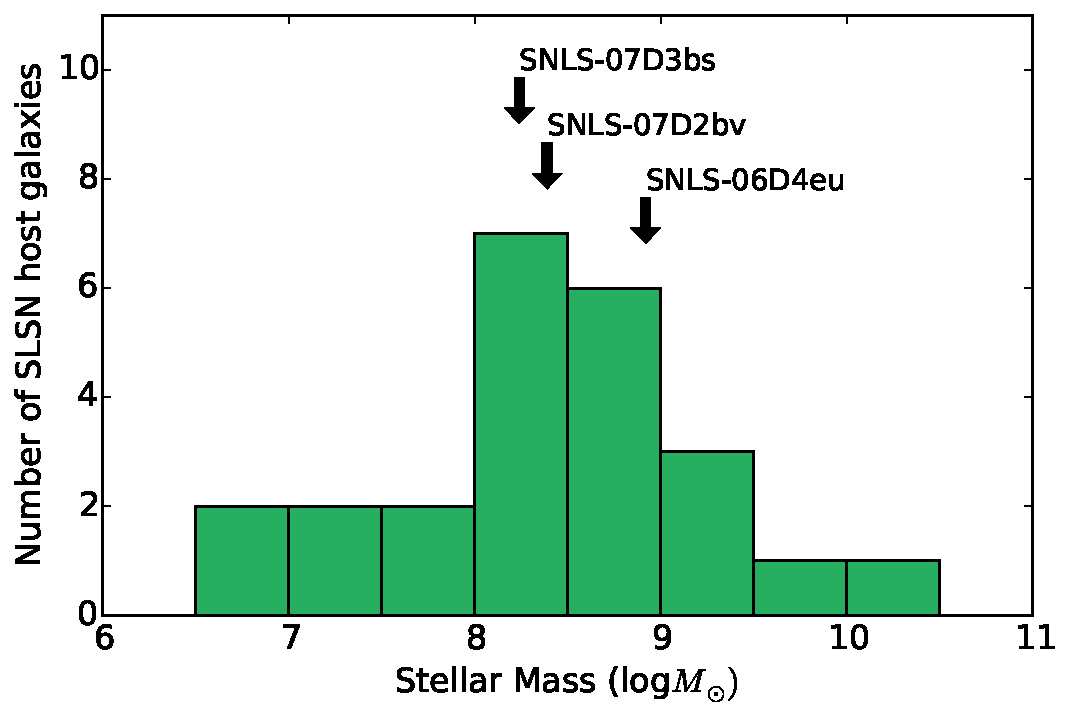
\includegraphics[width=\textwidth]{Figures/Chapter4/Galaxy}
\caption{The stellar mass distribution of SLSN host galaxies plotted using the data from \citet{Lunnan2014}, showing the consistency of SNLS07D3bs with the rest of the population. The lack of detections for the hosts of the high redshift candidates is consistent with being associated with low mass galaxies, found below the detection limit of SNLS at their redshifts.}
\label{fig:hosts}
\end{figure}
